\section{Space Policy}

\begin{sectionauthor}
    Dr. Lindsay DeMarchi (U.S. Congressional Fellow) \\
    Emma Louden (Yale University)
\end{sectionauthor}
\vspace{20pt}



\noindent Imagine playing a game without any rules. It would be chaotic, right? Similarly, space policy acts as the ``rulebook'' for space activities. With more countries and even private companies sending satellites, rovers, and astronauts into space, we need to ensure that everyone plays fair and safe.

\subsection{Aerospace/Astronautics}

As humans began to dream of reaching the stars, it became clear that rules were needed. The 1967 Outer Space Treaty, signed by many countries, laid the groundwork. This treaty states some fundamental principles:

\begin{itemize}
    \item Space is for Everyone: No country can claim ownership of the Moon or any other celestial body. Space is the ``common heritage of [hu]mankind.''
    \item Peaceful Purposes: Military activities, like placing nuclear weapons in space, are prohibited. Space should be a zone of peace.
    \item Liability and Responsibility: If a country launches an object into space, they're responsible for any damage it might cause, both in space and on Earth.
\end{itemize}

The United Nations (UN) plays a significant role in setting up these rules. They have a special committee called the ``Committee on the Peaceful Uses of Outer Space'' (or COPUOS for short). Members from different countries come together in this committee to discuss and agree on the best practices for space exploration. 

While the United Nations plays a pivotal role in creating global space rules, individual countries also have their own national space policies. These policies guide their space missions, research, and commercial activities.

Moreover, it's not just countries anymore! Private companies, like SpaceX and Blue Origin, are now major players in space exploration. They, too, must follow international and national space rules.


\vspace{15pt}

\textsc{Challenges and Considerations in Space Policy}\\

\vspace{-1cm}

\strut\hrulefill

\vspace{5pt}

\textbf{Space Traffic Management.} As more countries and private entities launch satellites and spacecraft, space is becoming crowded. Just like cars on a highway, these objects can collide if they're not carefully managed. 

To prevent accidents, we need a system to track all objects in space and predict their paths. This is similar to air traffic control for airplanes but on a much grander scale. Countries and organizations are working on creating ``rules of the road'' for space to ensure that all spacecraft can coexist without crashing into each other.

\textbf{Space Debris.} Over the years, many missions have left behind broken satellites, spent rocket stages, and even lost tools. These pieces of space junk can travel at speeds of up to 28,000 kilometers per hour! At such speeds, even a small piece of debris can cause significant damage to a satellite or space station. In fact, pieces larger than 10cm can mean the end of a mission entirely.

There are initiatives to track larger pieces of space debris and predict their orbits. Additionally, new missions are being designed to be ``cleaner,'' either by ensuring they burn up upon re-entry or by building mechanisms to remove them from orbit at the end of their life. Some companies and agencies are even exploring technologies to actively clean up space by capturing and de-orbiting old debris.

The issue of space debris requires top innovative minds, as moving junk to higher ``graveyard" orbits can simply duplicate the problem farther from the Earth, and burning up all debris in Earth's atmosphere can pollute the upper stratosphere with an imbalance of heavy metals. 

\textbf{Planetary Protection.} When we send rovers or astronauts to other planets or moons, there's a risk that Earth microbes could hitch a ride and contaminate these celestial bodies. This could jeopardize the search for alien life by making it hard to distinguish between local and Earth-born organisms. Conversely, if astronauts or probes return from these destinations, they could potentially bring back alien microbes that might be harmful to Earth's ecosystem.

Strict sterilization procedures are in place for spacecraft visiting sensitive destinations. For example, rovers destined for Mars undergo rigorous cleaning to minimize the risk of contamination. Similarly, protocols are being developed for safe return missions to ensure that any samples brought back are securely contained and studied without risk to our environment.

\textbf{Resource Utilization.} Celestial bodies, like asteroids and the Moon, are rich in resources that could be valuable for both space missions and use on Earth. However, unchecked mining could damage these environments and lead to conflicts over who has the right to these resources.

International agreements, like the Outer Space Treaty, state that the exploration and use of outer space shall be carried out for the benefit of all countries. This means that space resources should be used responsibly and equitably. Discussions are ongoing about how to regulate space mining to ensure that it's sustainable, doesn't harm the celestial environment, and benefits humanity as a whole. Most recent in this list is The Artemis Accords, an international partnership as we explore the Moon and other areas of deep space, such as asteroids. The signatories agree to maintain transparency in our science and guide to implement the obligations stated first in the Outer Space Treaty.

\subsection{Dark Sky Conservation}

Dark sky conservation can refer to a number of realms, depending on what you consider to be the ``sky." For some, dark skies hearken to our immediate atmosphere, and the phenomenon of ``noctalgia," or watching our stars disappear from an unnatural atmospheric glow or the scattering of artificial light at night (ALAN). For others, dark sky conservation extends from the surface of Earth to the deep recesses of space, and anything that interrupts our view of nature in between. 

As you've just learned, there are few laws governing outer space and the sky. Instead, the cutting edge of the conversation preceding additional policy is a series of ``best-practices" conversations, documents, and agreements working to set the tone for how we should proceed, regulate, or even \textit{think} about the sky. These conversations are like a wet clay, and \textbf{your voice matters.} 

\textbf{The Atmosphere} You may have noticed that there are some parts of the planet where you can barely see any stars at all, and others where you can see the whole Milky Way! That is because of ALAN and the large number of unshielded, unprotected lights humans use to illuminate the dark. The great thing about this form of light pollution is that it's immediately fixable. Just use proper lighting, et voila! The stars return!

Imagine trying to fill a cup of water using a pipe jetting out of your wall. Water would spurt everywhere, and you'd be lucky to catch any of it in your cup. Instead, we tend to use faucets such that we may easily direct the water into our vessels. Light should be treated the same way! In other words, solving ALAN doesn't mean turning all the lights off; it means directing light like a faucet. The next time you're high in a plane or on a rooftop, ask yourself whether or not it's necessary for photons from the ground to be reaching your eye. Could that be repaired with a simple cap on top of a naked light bulb?

The International Dark Sky Association (recently re-branded as ``Dark Sky International") is one international organization that seeks to educate and promote more conscious uses of proper lighting. Not only does better lighting reclaim our view of the night sky, but we save money, increase safety, save energy, and help critically affected wildlife. Think about it -- animals, plants, trees -- pretty much all life on Earth developed \textit{millions} of years in a cycle of daylight and natural darkness.

\textbf{From Satellites} One of the top 20 brightest stars in the sky is an artificial satellite. Currently, there are about 5,000 functioning satellites in orbit, but 530,000 are in various stages of planning, and that number is constantly changing! (Seriously, you should check for yourself what the current estimates are!)

Dark Sky International published their own list of five principles to preserve the quiet enjoyment of the night sky and protect the general public from the impacts of ``megaconstellations," or large swarms of satellites:
\begin{enumerate}
    \item Stewardship of the night sky is a shared responsibility that requires participation and consultation with all stakeholders.
    \item The cumulative impact on night sky brightness attributed to satellites does not exceed 10 percent above natural background levels.
    \item Maintained satellite brightness is below the threshold for detection by the unaided eye.
    \item Satellite visibility is an unusual occurrence.
    \item Launch schedules and orbital parameters are publicly available in advance.
\end{enumerate}

In addition to the general public, astronomers who take long exposures of the sky often find their data is tainted or ruined with bright satellite streaks. Though some companies, such as SpaceX, have agreed to paint their satellites darker, the fuselages themselves still block photons from reaching the Earth. This can be particularly harmful to transient astronomy and the world of cutting edge science, where we may not get a second chance to view an event.

The IAU CPS (or, the International Astronomical Union's Centre for the Protection of the Dark and Quiet Sky from Satellite Constellation Interference) is an international group of stakeholders with various ``hubs." These hubs are pillars that include Community Engagement, Policy, Industry, and Science, who all work together to compromise on the issue and suggest regulation and inform members of the public and industry. Their report and recommendations in a series ``Dark and Quiet Skies for Science and Society”  have been elevated to an agenda item in UN meetings on COPUOS. Additionally, NSF’s NOIRLab have held two conferences, summarized in proceedings called SATCON1 and SATCON2 they are invaluable touchstone documents that host recommendations for astronomers and industry alike, such that the negative impacts of satellites on astronomy can be mitigated.

\textbf{(Radio) Quiet Skies} Your Wi-Fi, your smart refrigerator, your car, and your cell phone all communicate via radio waves. In fact, so does everything else that uses satellites: banks, international trading ships, the military, and GPS! Oh, and your television broadcasts, too. The radio spectrum is broken up into wavelengths that can be registered through the ITU (International Telecommunication Union). As industry in space increases, so does the demand for radio wavelengths. Oftentimes, this overcrowding can create unintentional leakage and disrupt protected wavelengths, such as those reserved for astronomy. 

For perspective, the radio observatory called The Very Large Array (VLA) is sensitive enough to detect a flip-phone on Jupiter! Even if cell phones occupy bands adjacent to protected wavelengths and place their satellites on opposite sides of the Earth from the VLA, interference can spill over and be disruptive to science. Oftentimes, radio telescopes that observe low frequencies near the 5Ghz band feel their data is too noisy to warrant cleaning or further use. 

\begin{figure}[h!]
    \centering
    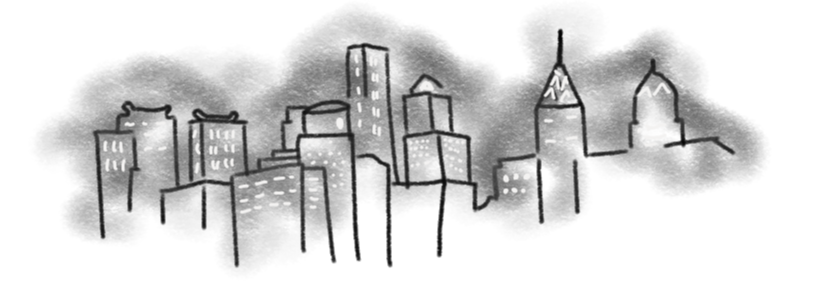
\includegraphics[width=\linewidth]{img/lightpollution.png}
    \caption{We can bring the Milky Way back to our cities. With proper lighting, even urban areas can see the night sky! }
    \label{fig:lightpollution}
\end{figure}